% =====================================================================
% Versión en español del artículo-perla de formalización.
% Estilo: técnico pero llano; guiado por preguntas (cada sección abre con una
% pregunta y viaja hasta su respuesta); cada afirmación argumentada; humildad;
% alcance enunciado con exactitud.
% =====================================================================
\documentclass[11pt]{article}
\usepackage[utf8]{inputenc}
\usepackage[T1]{fontenc}
\usepackage{lmodern}
\usepackage[spanish,es-noquoting]{babel}
\usepackage{amsmath,amssymb,amsthm,booktabs,graphicx,hyperref}
\usepackage{xurl}
\usepackage[table]{xcolor}
\definecolor{ggteal}{HTML}{1B6F8C}
\definecolor{ggband}{HTML}{DCE7EB}
\definecolor{ggamber}{HTML}{E08A1E}
\usepackage[margin=1in]{geometry}
\usepackage{microtype}
\setlength{\emergencystretch}{2em}
\graphicspath{{figures/}}
\renewcommand{\tablename}{Tabla}
\newtheorem{theorem}{Teorema}
\newtheorem{lemma}{Lema}
\newtheorem{definition}{Definición}
\newcommand{\lean}[1]{\texttt{\hyphenchar\font=`\- #1}}
\newcommand{\Z}{\mathbb{Z}}
\newcommand{\R}{\mathbb{R}}

\title{\bf De signos aleatorios a emparejamientos\\[3pt]
  \large\normalfont Una identidad de Godsil--Gutman, formalizada en Lean~4}
\author{Carles Mar\'in\thanks{Formalizado con asistencia de IA (Claude, Anthropic); la matemática y todas las afirmaciones son responsabilidad del autor. La metodología se discute en la Sección~\ref{sec:implications}.}\\[3pt]
  \normalsize Investigador independiente\\
  \normalsize \texttt{karlesmarin@gmail.com}}
\date{Junio de 2026}

\begin{document}
\maketitle

\begin{abstract}
Presento una formalización verificada por máquina, en Lean~4 / Mathlib, de la
identidad de Godsil--Gutman: el polinomio característico promedio de un signo
$\pm1$ uniformemente aleatorio de un grafo es su \emph{polinomio de
emparejamientos}. Por el camino formalizo el propio polinomio de emparejamientos
y su recurrencia de borrado, para la que no encontré formalización previa en
ningún asistente de demostración. Después aíslo el único ingrediente que
hace funcionar la prueba, un hecho de \emph{promediado de signos} sobre $\Z/2$
($\sum_{s=\pm1}s^{k}=2\,[k\text{ par}]$), y muestro que el \emph{mismo} lema
formal subyace a una segunda identidad, de nivel de momentos (el recuento de
paseos cerrados de paridad par de Chen--van~Dam--Bu). Por último formalizo la
descomposición espectral de Bilu--Linial de un $2$-levantamiento con signo, el
puente que conecta todo esto con los grafos de Ramanujan.
Soy deliberadamente preciso sobre qué está hecho y qué no: los teoremas
principales están libres de \lean{sorry} y dependen solo de los tres axiomas
estándar, pero la mitad profunda del programa de Marcus--Spielman--Srivastava
(raíces reales de Heilmann--Lieb, familias entrelazadas) está cartografiada, no
formalizada. Esto es una perla, no un hito; espero que sea una primera piedra
útil.
\end{abstract}

% ---------------------------------------------------------------
\section{Una pregunta sobre los signos}
\label{sec:intro}

Tome un grafo finito $G$ y ponga un signo, $+1$ o $-1$, en cada arista. La
\emph{matriz de adyacencia con signo} resultante $A_s$ tiene un polinomio
característico $\det(xI-A_s)$. Signos distintos dan polinomios distintos. Una
pregunta natural---y el punto de partida de un bello capítulo de la teoría
espectral de grafos---es:
\begin{quote}\itshape
  ¿qué se obtiene al promediar $\det(xI-A_s)$ sobre los $2^{|E|}$ signos?
\end{quote}
La respuesta, debida a Godsil y Gutman~\cite{GodsilGutman1981}, es llamativa: el
promedio es exactamente el \emph{polinomio de emparejamientos}
$\mu_G(x)=\sum_k(-1)^k m_k\,x^{n-2k}$, donde $m_k$ cuenta los emparejamientos de
$k$ aristas de $G$ (Figura~\ref{fig:gg}). Un promedio espectral sobre signos
aleatorios es igual a un recuento puramente combinatorio de emparejamientos.

\begin{figure}[t]
  \centering
  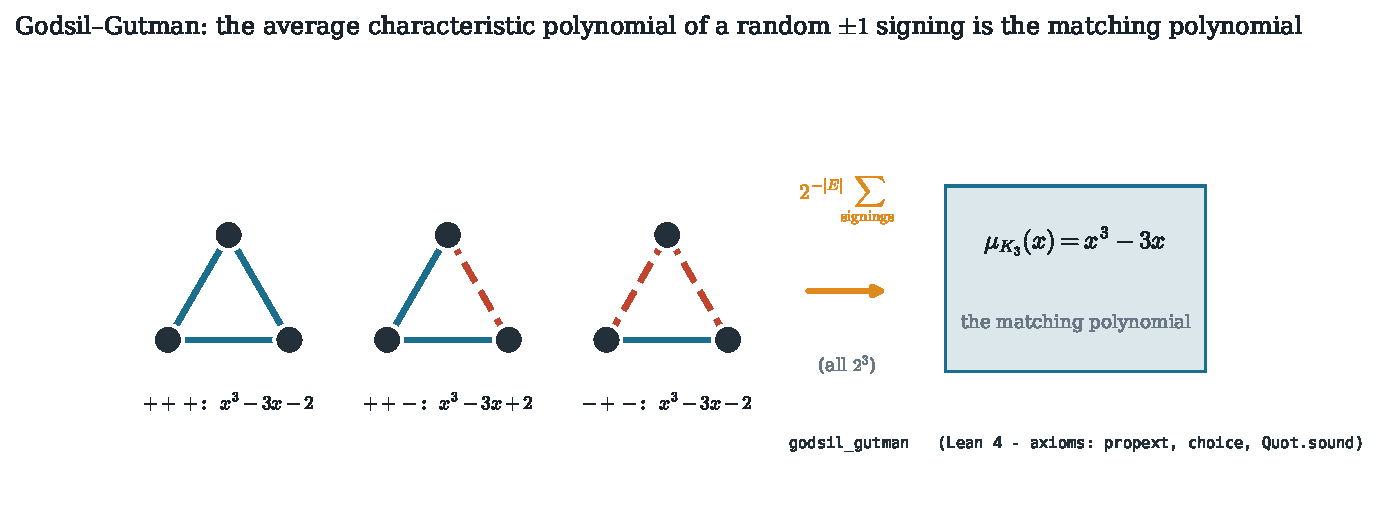
\includegraphics[width=\textwidth]{fig1_godsil_gutman.pdf}
  \caption{Godsil--Gutman sobre $K_3$: cada signo $\pm1$ (teal $+$, rojo
  discontinuo $-$) da un polinomio característico; su promedio es el polinomio de
  emparejamientos $\mu_{K_3}(x)=x^3-3x$. Verificado por máquina como
  \lean{godsil\_gutman}.}
  \label{fig:gg}
\end{figure}

¿Por qué debería importarle esto a alguien fuera de la teoría espectral de
grafos, y por qué formalizarlo? Dos razones recorren juntas este artículo.

\paragraph{Es la puerta a los grafos de Ramanujan.}
Un signo de $G$ es el mismo dato que un $2$-levantamiento (recubrimiento doble)
de $G$, y los autovalores ``nuevos'' del levantamiento son precisamente los
autovalores de $A_s$ (Bilu--Linial; Sección~\ref{sec:twolift}). Así que el
polinomio característico promedio de los autovalores nuevos es $\mu_G$. Heilmann
y Lieb~\cite{HeilmannLieb1972} probaron que las raíces de $\mu_G$ caen todas en
$[-2\sqrt{\Delta-1},\,2\sqrt{\Delta-1}]$---el umbral de Ramanujan
(Figura~\ref{fig:bound}). Marcus, Spielman y Srivastava~\cite{MSS2015a} usaron
después un argumento de familias entrelazadas para mostrar que \emph{algún} signo
logra un levantamiento cuyos autovalores nuevos están todos dentro de ese umbral,
probando la existencia de grafos de Ramanujan de todo grado. Godsil--Gutman es el
primer eslabón de esa cadena.

\begin{figure}[t]
  \centering
  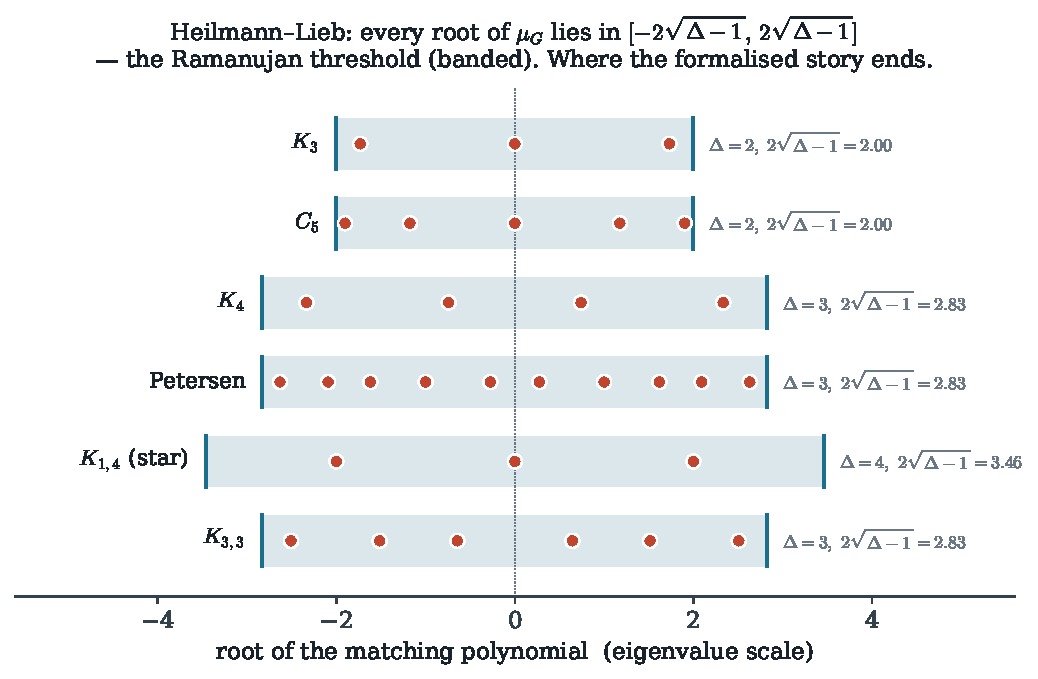
\includegraphics[width=\textwidth]{fig2_ramanujan_bound.pdf}
  \caption{Heilmann--Lieb: las raíces (calculadas) del polinomio de
  emparejamientos caen todas dentro de la banda
  $[-2\sqrt{\Delta-1},\,2\sqrt{\Delta-1}]$, el umbral de Ramanujan. Esta cota es
  el final del programa; aquí está cartografiada (Sección~\ref{sec:future}), aún
  no formalizada.}
  \label{fig:bound}
\end{figure}

\paragraph{Esconde un único patrón reutilizable.}
La prueba de Godsil--Gutman, cuando se mira de cerca, descansa sobre un hecho
diminuto: promediar un monomio de signos sobre $\pm1$ mata toda potencia impar y
duplica toda potencia par. Esto es una proyección de Fourier sobre $\Z/2$ y---esta
es la parte que me pareció digna de contar---el \emph{mismo} lema formal impulsa
una identidad aparentemente distinta, de nivel de momentos
(Sección~\ref{sec:engine}). La formalización convierte esa estructura compartida,
de un eslogan, en algo que el lector puede comprobar por su nombre.

\paragraph{Contribuciones.}
Aporto, todo en Lean~4 / Mathlib y todo libre de \lean{sorry} con
\lean{\#print axioms} reportando solo \lean{propext}, \lean{Classical.choice},
\lean{Quot.sound} (Tabla~\ref{tab:results}):
\begin{enumerate}\itemsep2pt
\item el polinomio de emparejamientos, el número de emparejamiento y la
  recurrencia de borrado $m_{k+1}(G)=m_{k+1}(G{-}v)+\sum_{u\sim v}m_k(G{-}v{-}u)$;
\item una prueba completa de la identidad de Godsil--Gutman (\lean{godsil\_gutman});
\item el motor de promediado de signos sobre $\Z/2$ y sus dos consumidores---
  Godsil--Gutman a nivel de polinomio característico y el núcleo de paseos
  cerrados de paridad par a nivel de momentos;
\item la factorización de Bilu--Linial del polinomio característico del
  $2$-levantamiento, \lean{charpoly\_twoLift}.
\end{enumerate}
Soy igual de explícito sobre la frontera del trabajo
(Sección~\ref{sec:future}): Heilmann--Lieb y el paso de familias entrelazadas
están cartografiados en detalle pero no formalizados.

% Tablas (versión en español) para el artículo-perla de formalización.
% Requiere \usepackage{booktabs,amsmath,amssymb} y \usepackage[table]{xcolor}
% en el preámbulo, más los colores ggteal / ggband.

% ---------- Tabla 1: resultados formalizados ----------
\begin{table}[t]
  \centering
  \small
  \arrayrulecolor{ggteal}
  \caption{Los resultados formalizados (Lean~4 / Mathlib). Todos los teoremas
  están libres de \texttt{sorry} y son no vacíos; \texttt{\#print axioms} reporta
  solo \texttt{propext}, \texttt{Classical.choice}, \texttt{Quot.sound}.}
  \label{tab:results}
  \begin{tabular}{@{}llc@{}}
    \toprule
    \rowcolor{ggteal}
    \textcolor{white}{\textbf{Nombre Lean}} & \textcolor{white}{\textbf{Enunciado}} & \textcolor{white}{\textbf{Estado}} \\
    \midrule
    \rowcolor{ggband}
    \texttt{godsil\_gutman} & $\sum_{\mathrm{cfg}}\det(xI-A_{\mathrm{cfg}})=\#\mathrm{cfg}\cdot\mu_G$ & probado \\
    \texttt{matchingPoly} (+infra) & $\mu_G=\sum_k(-1)^k m_k\,x^{n-2k}$ (sin formalización previa) & definido \\
    \rowcolor{ggband}
    \texttt{matchingNumber\_recurrence} & $m_{k+1}(G)=m_{k+1}(G{-}v)+\sum_{u\sim v} m_k(G{-}v{-}u)$ & probado \\
    \texttt{charpoly\_twoLift} & $\det\!\bigl(xI-\bigl[\begin{smallmatrix}B&C\\C&B\end{smallmatrix}\bigr]\bigr)=\mu_{B+C}\,\mu_{B-C}$ & probado \\
    \rowcolor{ggband}
    \texttt{signAvg\_ne\_zero\_iff} & el signo-monomio sobrevive $\iff$ multiplicidades pares & probado \\
    \texttt{sum\_signOf\_prod\_pow} & núcleo de proyección de paridad $\mathbb{Z}/2$ (nivel de momentos) & probado \\
    \midrule
    \emph{Heilmann--Lieb} & $\text{raíces}(\mu_G)\subseteq[-2\sqrt{\Delta-1},\,2\sqrt{\Delta-1}]$ & futuro \\
    \rowcolor{ggband}
    \emph{familias entrelazadas} & $\exists$ signo con $\lambda_{\max}\le\lambda_{\max}(\overline{\,\cdot\,})$ & futuro \\
    \bottomrule
  \end{tabular}
  \arrayrulecolor{black}
\end{table}

% ---------- Tabla 2: comprobaciones numéricas ----------
\begin{table}[t]
  \centering
  \small
  \arrayrulecolor{ggteal}
  \caption{Comprobaciones numéricas de las identidades formalizadas (SymPy,
  exacto). Izquierda: el polinomio característico promedio sobre todos los signos
  $\pm1$ es igual a $\mu_G$ (Godsil--Gutman). Derecha: el $d$-ésimo momento
  espectral promedio es igual al número de paseos cerrados de paridad par (aquí
  $d=4$).}
  \label{tab:checks}
  \begin{tabular}{@{}llcc@{}}
    \toprule
    \rowcolor{ggteal}
    \textcolor{white}{\textbf{$G$}} & \textcolor{white}{\textbf{$2^{-|E|}\!\sum_{\mathrm{signos}}\det(xI-A_s)$}} & \textcolor{white}{\textbf{$=\mu_G$?}} & \textcolor{white}{\textbf{$\overline{\mathrm{tr}(A_s^{4})}=P_4$}} \\
    \midrule
    \rowcolor{ggband}
    $K_3$ & $x^{3}-3x$         & $\checkmark$ & $18$ \\
    $C_4$ & $x^{4}-4x^{2}+2$   & $\checkmark$ & $24$ \\
    \rowcolor{ggband}
    $C_5$ & $x^{5}-5x^{3}+5x$  & $\checkmark$ & $30$ \\
    $K_4$ & $x^{4}-6x^{2}+3$   & $\checkmark$ & $60$ \\
    \rowcolor{ggband}
    $K_{3,3}$ & $x^{6}-9x^{4}+18x^{2}-6$ & $\checkmark$ & $90$ \\
    Petersen & $x^{10}-15x^{8}+75x^{6}-145x^{4}+90x^{2}-6$ & $\checkmark$ & $150$ \\
    \bottomrule
  \end{tabular}
  \arrayrulecolor{black}
\end{table}


% ---------------------------------------------------------------
\section{¿Qué se está promediando exactamente?}
\label{sec:setting}

Antes de que una máquina pueda comprobar nada, los objetos deben quedar fijados.
Trabajo sobre un tipo de vértices finito arbitrario $V$.

\begin{definition}[Adyacencia con signo]
Un signo es una función $\mathrm{cfg}\colon \mathrm{Sym2}\,V\to\mathrm{Bool}$
sobre los pares no ordenados. La matriz de adyacencia con signo
$A_{\mathrm{cfg}}$ es la matriz real simétrica que vale $\pm1$ en las aristas
(según $\mathrm{cfg}$) y $0$ en el resto.
\end{definition}

Una sutileza pequeña pero honesta aflora de inmediato, y conviene enunciarla con
claridad en lugar de ocultarla. Dejo que $\mathrm{cfg}$ recorra \emph{todos} los
pares no ordenados, no solo las aristas; los bits de no-arista simplemente son
ignorados por $A_{\mathrm{cfg}}$. En consecuencia cada signo genuino se cuenta
$2^{|\mathrm{Sym2}\,V|-|E|}$ veces, y mi teorema dice
\[
  \boxed{\;\sum_{\mathrm{cfg}}\det(xI-A_{\mathrm{cfg}})
  \;=\;\bigl(\#\mathrm{cfg}\bigr)\cdot \mu_G\;},
  \qquad \#\mathrm{cfg}=2^{|\mathrm{Sym2}\,V|}.
\]
Dividir por $\#\mathrm{cfg}$ recupera exactamente el promedio por aristas de los
libros de texto $2^{-|E|}\sum_{\text{signos}}=\mu_G$; los bits redundantes de
no-arista se cancelan. Elegí la formulación sobre todos los pares porque hace que
la estructura de Fourier sobre $\Z/2$ de la prueba (Sección~\ref{sec:engine}) sea
uniforme sobre todo el tipo de índices, al precio de esta única observación de
contabilidad.

\begin{definition}[Polinomio de emparejamientos]
$\mu_G(x)=\sum_{k=0}^{\lfloor n/2\rfloor}(-1)^k m_k(G)\,x^{\,n-2k}$, donde
$m_k(G)$ es el número de subconjuntos de $k$ aristas mutuamente disjuntas en
vértices y $n=|V|$.
\end{definition}

Mathlib tiene una teoría rica de grafos simples y de polinomios característicos,
pero ningún polinomio de emparejamientos; construirlo (y probar su recurrencia de
borrado) fue un prerrequisito, y no encontré formalización previa de él en
ningún asistente de demostración.\footnote{Busqué una formalización
previa del polinomio de emparejamientos en los principales asistentes de
demostración (junio de 2026): Mathlib (Lean), el Archive of Formal Proofs
(Isabelle), el ecosistema Coq/MathComp, HOL~Light y Agda. Los
\emph{emparejamientos} como conjuntos de aristas sí están formalizados---por
ejemplo el emparejamiento de cardinalidad máxima y el estable en el AFP, y el
teorema de Hall en Lean y Coq---pero no encontré formalización del \emph{polinomio}
de emparejamientos $\mu_G$, sus coeficientes $m_k$, ni su recurrencia de borrado.
La búsqueda fue de buena fe, no exhaustiva; de ahí ``hasta donde sé''.}

% ---------------------------------------------------------------
\section{Cómo una máquina prueba Godsil--Gutman}
\label{sec:gg}

La prueba clásica de un párrafo desarrolla $\det(xI-A_{\mathrm{cfg}})$ sobre
permutaciones, suma sobre los signos y observa que solo sobreviven las
permutaciones que son \emph{involuciones hechas de aristas}---es decir,
emparejamientos. Convertir ese párrafo en una prueba verificada significó hacer
explícito cada ``obsérvese que''. La arquitectura es una tubería corta; la
esbozo y señalo los dos lugares que opusieron resistencia.

\paragraph{Solo sobreviven las involuciones de aristas.}
El determinante es $\sum_{\sigma}\mathrm{sign}(\sigma)\prod_i(\cdots)$; al sumar
sobre los signos, la contribución de una permutación $\sigma$ es, salvo
signo y una potencia de $x$, una suma interna sobre los signos de un producto a lo
largo del soporte de $\sigma$. Pruebo (\lean{innerSum\_eq\_ite}) que esa suma
interna vale $\#\mathrm{cfg}$ cuando $\sigma$ es una involución de aristas
($\sigma^2=1$ con cada $2$-ciclo una arista) y $0$ en caso contrario. El
``$0$ en caso contrario'' es exactamente la cancelación sobre $\Z/2$: una
permutación con una arista no emparejada aporta un signo que se promedia hasta
desaparecer.

\paragraph{Las involuciones de aristas son emparejamientos.}
Las permutaciones supervivientes están en biyección con los emparejamientos: una
involución de aristas $\sigma$ va a su conjunto de aristas-$2$-ciclo, y un
emparejamiento vuelve a la involución que intercambia los extremos de cada arista.
Construyo esta biyección explícitamente---\lean{matchingOfPerm} en un sentido,
\lean{permOfMatching} en el otro---y pruebo ambos viajes de ida y vuelta. Una
sorpresa agradable fue que la aplicación inversa es \emph{irrelevante en la
prueba} respecto de la hipótesis de emparejamiento (el dato de la permutación
depende solo del emparejamiento, no de la prueba de que lo sea), lo que permitió
descargar limpiamente las obligaciones de \lean{Finset.sum\_bij'}.

\paragraph{Los dos puntos difíciles.}
Primero, una coerción: pasar $(-1)^k$ del grupo de unidades $\Z^\times$ a través
de $\Z$ hasta $\R[x]$. La reescritura natural de Mathlib
(\lean{Units.val\_pow\_eq\_pow\_val}) es definicionalmente un no-op y falla
silenciosamente al reescribir; necesité una inducción corta
(\lean{intCast\_units\_neg\_one\_pow}). Segundo, el reensamblaje final requirió
una suma fibrada sobre el tamaño del emparejamiento con un término de frontera,
tratado con \lean{Finset.sum\_fiberwise\_of\_maps\_to} y la cota de tamaño de
emparejamiento $2k\le n$. Ninguno es profundo, pero ambos son el tipo de fricción
que una formalización debe absorber y sobre la que un artículo debería ser
honesto.

El resultado, \lean{godsil\_gutman}, es el enunciado preciso de la
Sección~\ref{sec:setting}, verificado por máquina.

% ---------------------------------------------------------------
\section{El motor de debajo: un hecho sobre $\Z/2$, dos identidades}
\label{sec:engine}

¿Por qué ocurre la cancelación de la Sección~\ref{sec:gg}? Por un único hecho
aritmético sobre los signos:
\[
  \boxed{\;\sum_{s\in\{\pm1\}} s^{\,k}
  \;=\;
  \begin{cases} 2 & k\text{ par},\\ 0 & k\text{ impar}\end{cases}\;}.
\]
En Lean esto son dos lemas de una línea (\lean{sum\_signOf\_pow\_eq\_two\_of\_even}
y \lean{\_zero\_of\_odd}). Promediar un producto de signos de aristas sobre todos
los signos se factoriza, por \lean{Fintype.prod\_sum}, en un producto de estas
sumas por arista; así que \emph{un monomio de signos sobrevive al promedio si y
solo si toda multiplicidad de arista es par}. Empaqueto esto como la compuerta de
paridad (\lean{signAvg\_ne\_zero\_iff}; Figura~\ref{fig:engine}).

\begin{figure}[t]
  \centering
  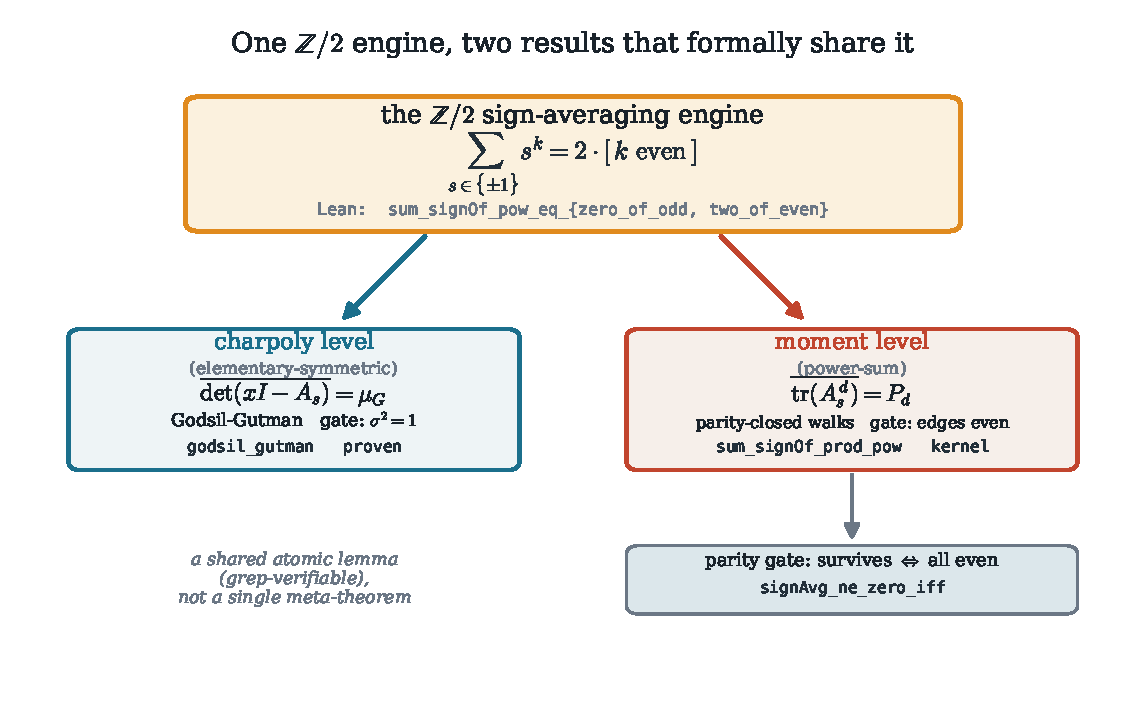
\includegraphics[width=0.92\textwidth]{fig3_zmod2_principle.pdf}
  \caption{Un único hecho de promediado de signos sobre $\Z/2$
  (\lean{sum\_signOf\_pow}) alimenta tanto Godsil--Gutman (nivel de polinomio
  característico) como el núcleo de paseos cerrados de paridad par (nivel de
  momentos). La unificación es un lema atómico compartido, visible en el grafo de
  dependencias---no un único meta-teorema; la compuerta de paridad
  (\lean{signAvg\_ne\_zero\_iff}) está ella misma aguas abajo del núcleo de
  momentos.}
  \label{fig:engine}
\end{figure}

Aquí está la parte que encuentro genuinamente grata, y la enuncio con cuidado para
evitar sobreafirmar. Los mismísimos lemas por arista impulsan una \emph{segunda}
identidad, en apariencia no relacionada. Chen, van~Dam y
Bu~\cite{ChenVanDamBu2023} observan que el $d$-ésimo momento espectral promedio de
un grafo con signo cuenta sus \emph{paseos cerrados de paridad par} (paseos
cerrados que usan cada arista un número par de veces). A nivel de funciones
simétricas elementales se obtiene Godsil--Gutman; a nivel de sumas de potencias se
obtiene el recuento de paseos cerrados de paridad par. Son dos lecturas de la
misma proyección sobre $\Z/2$. Formalizo el núcleo algebraico de la segunda
identidad (\lean{sum\_signOf\_prod\_pow})---su forma completa de recuento de paseos
necesita infraestructura de paseos de la que Mathlib carece, que no reclamo.

\paragraph{Un punto de honestidad intelectual.}
La unificación aquí es real pero modesta, y la describo con exactitud. \emph{No}
probé un único meta-teorema del que ambos resultados sean corolarios. Lo que es
cierto---y formalmente comprobable por su nombre---es que ambas pruebas invocan
los \emph{mismos} lemas atómicos \lean{sum\_signOf\_pow\_eq\_*}. La estructura
compartida vive en el grafo de dependencias, no en un enunciado grandioso, y la
Figura~\ref{fig:engine} lo dibuja así.

% ---------------------------------------------------------------
\section{El puente a Ramanujan: los $2$-levantamientos}
\label{sec:twolift}

¿Qué tiene que ver todo esto con los expansores? El enlace es el
$2$-levantamiento. Un signo $s$ de $G$ determina un recubrimiento doble $G_s$ cuya
matriz de adyacencia tiene la forma en bloques
$\bigl[\begin{smallmatrix}A_+&A_-\\A_-&A_+\end{smallmatrix}\bigr]$, con $A_+,A_-$
las partes de aristas positivas y negativas. Formalizo la descomposición espectral
de esta matriz en bloques (\lean{charpoly\_twoLift}):
\[
  \boxed{\;\det\!\Bigl(xI-\begin{bmatrix}B&C\\ C&B\end{bmatrix}\Bigr)
  \;=\;\det(xI-(B{+}C))\cdot\det(xI-(B{-}C))\;},
\]
probada conjugando con la involución
$\bigl[\begin{smallmatrix}1&1\\1&-1\end{smallmatrix}\bigr]$ (que eleva al cuadrado
$2I$) a la forma diagonal por bloques. Con $B{+}C=A$ la adyacencia ordinaria y
$B{-}C=A_s$ la de signo, esto dice que el espectro del levantamiento es
$\mathrm{spec}(A)\uplus\mathrm{spec}(A_s)$: los autovalores \emph{nuevos} son
exactamente los de la matriz de adyacencia con signo. Así que Godsil--Gutman es la
afirmación de que su polinomio característico promedio es $\mu_G$---y Heilmann--Lieb
es la afirmación de que las raíces de $\mu_G$ respetan el umbral de Ramanujan.

Tengo cuidado de decir qué formalicé: el \emph{álgebra lineal} del
$2$-levantamiento (la identidad matricial de arriba), no la construcción
grafo-teórica del $2$-levantamiento. Esa es la pieza correcta, pero es un teorema
matricial con una lectura de grafos, y lo presento como tal.

% ---------------------------------------------------------------
\section{Cómo acaba la historia, y dónde me detuve}
\label{sec:future}

Sería deshonesto fingir que llegué al final. No lo hice. Pero puedo
cartografiarlo con precisión, porque el catálogo de lo que queda es corto y la
ruta es clásica.
\begin{enumerate}\itemsep2pt
\item[$\checkmark$] Godsil--Gutman (polinomio característico promedio $=\mu_G$).
\item[$\checkmark$] El puente del $2$-levantamiento (autovalores nuevos $=$
  autovalores con signo).
\item[$\checkmark$] El motor sobre $\Z/2$ que ata el lado espectral con el
  combinatorio.
\item[$\circ$] \textbf{Heilmann--Lieb}: $\text{raíces}(\mu_G)\subseteq
  [-2\sqrt{\Delta-1},2\sqrt{\Delta-1}]$. La ruta limpia es el árbol de caminos de
  Godsil: $\mu_G$ divide el polinomio de emparejamientos del árbol de caminos
  $T(G,u)$; $T$ es un bosque, sobre el que el polinomio de emparejamientos
  \emph{es igual} al polinomio característico (los signos son triviales por gauge),
  luego tiene raíces reales con la cota de radio espectral de árbol
  $2\sqrt{\Delta-1}$. Esto da las raíces reales y la cota de un golpe, y no
  necesita maquinaria externa de entrelazado.
\item[$\circ$] \textbf{Familias entrelazadas}~\cite{MSS2015a}: la familia
  $\{\det(xI-A_s)\}_s$ es entrelazada, así que la raíz mayor de algún miembro es a
  lo sumo la raíz mayor del promedio $\mu_G$, que es $\le2\sqrt{\Delta-1}$.
\item[$\circ$] De ahí existe un $2$-levantamiento de Ramanujan, y los grafos de
  Ramanujan de todo grado se siguen iterando.
\end{enumerate}
Los pasos~4--6 son una empresa de varios meses; una comprobación de la literatura
(Mathlib más una búsqueda en la web) no encontró formalización previa de
Heilmann--Lieb ni del polinomio de emparejamientos en ningún prover, así que el
camino está sin desgastar pero también sin construir. Creo que la contribución
honesta de este artículo es haber colocado, y verificado, las primeras piedras del
pavimento, y haber dibujado el resto del mapa a escala.

% ---------------------------------------------------------------
\section{La siguiente piedra: una propuesta de árbol de caminos}
\label{sec:proposal}

El mapa de la Sección~\ref{sec:future} nombra dos pasos sin construir. No cuestan
lo mismo, y confundirlos sería un flaco favor a quien decida qué hacer a
continuación. Así que hago la pregunta más afilada:

\begin{quote}\itshape
  ¿cuál es el \emph{menor} paso siguiente que convierte un trozo del mapa en
  carretera real---y cuánta carretera compra?
\end{quote}

Mi respuesta es Heilmann--Lieb vía el \emph{árbol de caminos} de Godsil, y creo
que es una ganga notable: una única construcción clásica que entrega a la vez las
raíces reales y la cota de Ramanujan, sin maquinaria de entrelazado. Aquí está el
plan, con detalle suficiente para empezar.

\paragraph{La construcción.}
Fije un vértice $u$ de $G$. El árbol de caminos $T(G,u)$ de Godsil es el árbol
cuyos vértices son los caminos en $G$ que parten de $u$, con un camino unido a
otro cuando lo extiende por una sola arista (Figura~\ref{fig:pathtree}). Es un
bosque finito, y carga toda la prueba sobre dos hechos.

\begin{figure}[t]
  \centering
  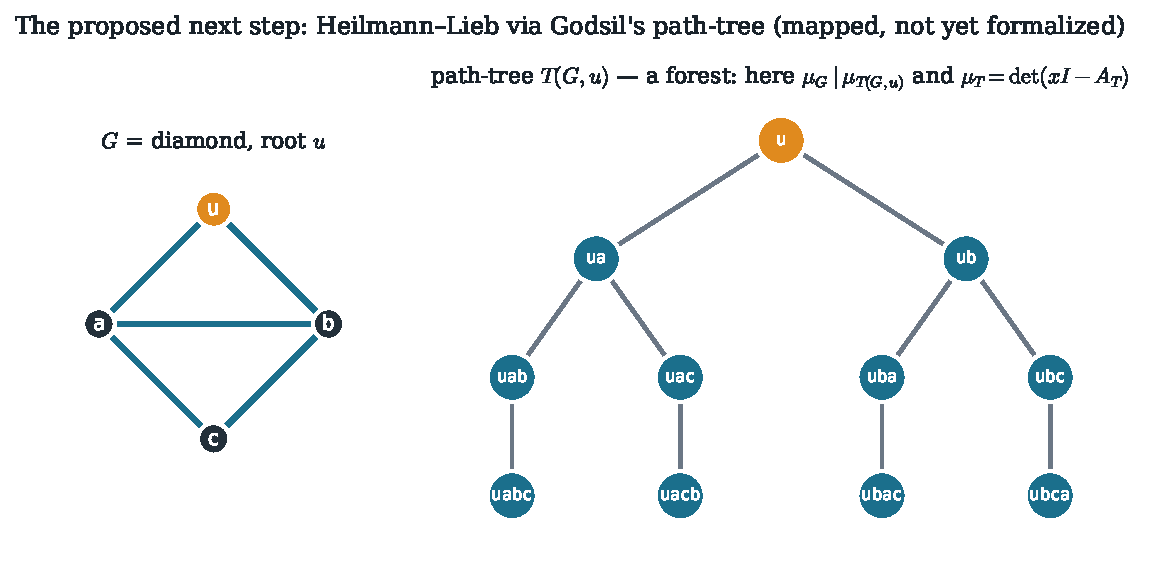
\includegraphics[width=\textwidth]{fig4_path_tree.pdf}
  \caption{El árbol de caminos $T(G,u)$ de Godsil del diamante $G$ (raíz $u$, en
  ámbar): sus vértices son los caminos de $G$ que parten de $u$, unidos cuando uno
  extiende al otro por una arista. $T(G,u)$ es un bosque, así que sobre él el
  polinomio de emparejamientos \emph{es igual} al polinomio característico de la
  matriz de adyacencia; y $\mu_G$ divide a $\mu_{T(G,u)}$. Estos dos hechos
  entregan Heilmann--Lieb. La construcción está cartografiada aquí, aún no
  formalizada.}
  \label{fig:pathtree}
\end{figure}

\paragraph{Los dos hechos que hacen el trabajo.}
\begin{enumerate}\itemsep2pt
\item[(i)] \textbf{Divisibilidad.} $\mu_G(x)$ divide a $\mu_{T(G,u)}(x)$ (Godsil).
  El polinomio de emparejamientos del árbol de caminos es un múltiplo del que nos
  importa, así que cualquier cota de raíces para $T$ se transfiere a $G$.
\item[(ii)] \textbf{Los bosques son triviales por gauge.} Sobre un bosque, el
  polinomio de emparejamientos \emph{es igual} al polinomio característico de la
  matriz de adyacencia: un árbol no tiene ciclos pares que obstruyan un cambio
  global de signo, así que los signos se pueden eliminar por gauge. Luego
  $\mu_{T(G,u)}$ es el polinomio característico de una matriz real simétrica, por
  tanto de raíces reales; y el radio espectral de un árbol de grado máximo
  $\Delta$ es a lo sumo $2\sqrt{\Delta-1}$.
\end{enumerate}
Junte (i) y (ii) y $\mu_G$ tiene raíces reales, todas en
$[-2\sqrt{\Delta-1},\,2\sqrt{\Delta-1}]$---Heilmann--Lieb, el umbral de Ramanujan,
de un golpe. Por eso el árbol de caminos es la piedra correcta y no solo \emph{una}
piedra: colapsa dos afirmaciones analíticas de aspecto separado en una sola
construcción combinatoria más hechos espectrales estándar que Mathlib ya tiene.

\paragraph{Lo que ya está en la mano, y lo que falta.}
El polinomio de emparejamientos y su recurrencia de borrado---el motor de toda
inducción sobre el árbol de caminos---son exactamente lo que este artículo
formaliza, así que la propuesta no parte de cero. Lo que a Mathlib todavía le
falta, y lo que un trabajo posterior debe construir, es: la propia construcción
del árbol de caminos (como un \lean{SimpleGraph} sobre un tipo de caminos); el
lema de divisibilidad~(i), cuya prueba de libro de texto es una inducción sobre la
recurrencia de borrado; y la identidad de bosque~(ii). Señalo una fricción
concreta que ya encontré y que este paso volverá a encontrar: la recurrencia del
número de emparejamiento tiene un caso de frontera ($m_N$ de un grafo tras borrar
dos vértices adyacentes se anula) que necesita un pequeño lema de vértices
aislados para descargarse limpiamente---menor, pero el tipo de detalle que una
formalización no puede pasar por alto.

\paragraph{Una invitación abierta.}
Lo enuncio como propuesta, no como resultado: ni (i), ni (ii), ni el propio árbol
de caminos están aún formalizados, y no los reclamo. Pero la ruta es clásica, los
prerrequisitos ya están en su sitio, y la recompensa---el primer Heilmann--Lieb
verificado por máquina---está bien definida. Si este artículo tiene una secuela,
esta es su primera frase.

% ---------------------------------------------------------------
\section{Implicaciones}
\label{sec:implications}

¿Para qué podría servir esta pequeña pieza de trabajo? Enumero tres clases de
implicación, en orden decreciente de cuán confiadamente puedo reclamarlas, y un
apunte metodológico.

\paragraph{Bloques de construcción certificados y reutilizables.}
El polinomio de emparejamientos, su recurrencia de borrado, la matriz de
adyacencia con signo y la factorización del polinomio característico del
$2$-levantamiento están ahora verificados por máquina y disponibles para
cualquiera que trabaje con emparejamientos o espectros de grafos con signo en un
asistente de demostración; Mathlib no tenía ninguno de ellos. En concreto, estas
son exactamente las piezas sobre las que se construiría una formalización futura:
Heilmann--Lieb vía el árbol de caminos de Godsil (Sección~\ref{sec:future})
reutiliza directamente el polinomio de emparejamientos y su recurrencia; el
teorema de estructura de Gallai--Edmonds y el polinomio de independencia se apoyan
en la misma infraestructura combinatoria; y el promedio de adyacencia con signo es
la receta precisa que hay detrás del más amplio \emph{método de polinomios
entrelazados}---la mismísima técnica que Marcus, Spielman y Srivastava usaron para
zanjar el problema de Kadison--Singer~\cite{MSS2015b}. Los lemas de promediado de
signos sobre $\Z/2$ son diminutos, pero el artículo muestra que son reutilizables
en dos niveles (simétrico-elemental y suma de potencias), y espero que reaparezcan
donde quiera que aparezca un polinomio característico esperado sobre signos
$\pm1$. Esta es la implicación que puedo afirmar con más firmeza: un puñado de
fundamentos nuevos y certificados.

\paragraph{Un peldaño hacia la existencia de Ramanujan formalizada.}
El teorema de Marcus, Spielman y Srivastava sobre grafos de Ramanujan de todo
grado es célebre, y, que yo sepa, ningún asistente lo ha abordado aún. Este artículo
formaliza su mitad estructural y cartografía la mitad analítica
(Sección~\ref{sec:future}) a escala. Si el hito llegara a construirse, estos son
fundamentos sobre los que apoyarse, y el mapa puede ahorrar a quien siga la
búsqueda bibliográfica que tuve que hacer.

\paragraph{La matemática, con una nota de cautela.}
Los grafos de Ramanujan y los expansores no son curiosidades abstractas: sostienen
códigos correctores de errores (códigos LDPC y de expansor), la desaleatorización
(el algoritmo en espacio logarítmico de Reingold para la conexión no dirigida usa
paseos sobre expansores), solucionadores rápidos del laplaciano, funciones hash
criptográficas construidas a partir de grafos de isogenias/expansores, y redes de
comunicación robustas---por eso importa el teorema subyacente. Soy cauto, sin
embargo, a la hora de tomar prestada esa importancia para este artículo.
Formalizar una identidad fundacional no entrega por sí solo un código ni una red;
su valor está en los fundamentos certificados y en el creciente corpus de
matemática formalizada, no en una aplicación inmediata. Reclamo lo primero y no lo
segundo.

\paragraph{Un apunte metodológico.}
Este desarrollo se llevó a cabo con un sistema de IA como instrumento de
investigación: propuso definiciones, lemas y tácticas, y un bucle de
compilación-como-oráculo verificó o rechazó cada uno contra el núcleo. La
contabilidad cuidadosa de este artículo---cada afirmación dimensionada a
exactamente lo que se probó, las limitaciones enunciadas con tanta llaneza como
los resultados---es ella misma parte de lo que espero que el trabajo ilustre: que
la formalización asistida por IA puede evitar la sobreafirmación que el método
invita, precisamente porque el asistente de demostración, no el asistente, tiene
la última palabra.

% ---------------------------------------------------------------
\section{Trabajo relacionado}
\label{sec:related}

La matemática es clásica: Godsil--Gutman~\cite{GodsilGutman1981},
Heilmann--Lieb~\cite{HeilmannLieb1972}, el programa de
Marcus--Spielman--Srivastava~\cite{MSS2015a,MSS2015b}, y el cuadro del
$2$-levantamiento / Bilu--Linial que lo subyace; el compañero de nivel de momentos
es reciente~\cite{ChenVanDamBu2023}. Por el lado de la formalización,
Mathlib~\cite{Mathlib2020} proporciona grafos simples y polinomios
característicos, pero ni el polinomio de emparejamientos ni la teoría espectral de
grafos con signo. El desarrollo se inscribe en una línea creciente de
formalizaciones de combinatoria en Lean---el teorema del matrimonio de
Hall~\cite{GusakovMehtaMiller2021}, el teorema de
Kruskal--Katona~\cite{Mehta2022KruskalKatona}, el lema de regularidad de
Szemer\'edi~\cite{DilliesMehta2022}, y perlas de demostración del mismo
espíritu~\cite{Mehta2023Sharkovsky}---ninguna de las cuales toca los polinomios de
emparejamientos ni los espectros de grafos con signo. El instrumental de
entrelazado \texttt{RealRooted} de PerAlexandersson es una base de código de
investigación, no una biblioteca pulida, y no incluye el polinomio de
emparejamientos; mi ruta planeada del árbol de caminos
(Sección~\ref{sec:proposal}) lo esquiva. No tengo constancia de ningún tratamiento
previo verificado por máquina de estos resultados.

% ---------------------------------------------------------------
\section{Conclusión}

Partí de una pregunta sencilla---¿cuál es el polinomio característico promedio de
un signo aleatorio?---y la seguí, en un asistente de demostración, hasta una
respuesta completa y verificada (Godsil--Gutman), hasta el pequeño hecho sobre
$\Z/2$ que la hace funcionar, hasta una segunda identidad que comparte ese hecho, y
hasta el puente matricial que lo apunta todo hacia los grafos de Ramanujan.
Ninguno de estos resultados es matemática nueva; la contribución es que ahora están
verificados por máquina, que el polinomio de emparejamientos está ahora
disponible en un prover donde no encontré formalización previa de él, y que el
motor compartido es visible en el grafo de dependencias
en lugar de afirmado. La mitad profunda de la historia---Heilmann--Lieb y las
familias entrelazadas---sigue por delante de mí, cartografiada pero sin construir.
Ofrezco esto como una perla y una invitación.

\paragraph{Artefactos.} Todas las fuentes Lean (libres de \lean{sorry},
dependiendo solo de los tres axiomas estándar; véase la Tabla~\ref{tab:results}),
las figuras de este artículo y las comprobaciones numéricas de la
Tabla~\ref{tab:checks} están disponibles en:
\begin{center}
\url{https://github.com/karlesmarin/godsil-gutman-lean}\\[2pt]
archivado en \textsc{doi}~\href{https://doi.org/10.5281/zenodo.20517350}{10.5281/zenodo.20517350}
\end{center}

\bibliographystyle{plain}
\bibliography{references}

\end{document}
